\section{Applying LSTM on Lorenz-datasets} \label{sec3}
	\subsection{Lorenz-63}
	\newcommand{\SixtyThreePath}{Results/Lorenz-63/Figures/RNN-lstm-RDIM_3-N_used_50000-NUM-LAY_1-SIZE-LAY_100-ACT_tanh-ISH_statefull-SL_8-PL_4-LR_0.0001-DKP_1.0-ZKP_1.0-HSPL_300-IPL_200-NL_1-WID_0}
	\newcommand{\SixtyThreePathIndexOne}{33278}
	\newcommand{\SixtyThreePathIndexTwo}{45336}
	
	\begin{figure}[h]
		\centering
		\begin{subfigure}[b]{0.45\textwidth}
			\includegraphics[width=\textwidth]{../\SixtyThreePath/Loss_total_log.png}
			\caption{Training and validation loss}
			\label{63:loss}
		\end{subfigure}
		\begin{subfigure}[b]{0.45\textwidth}
			\includegraphics[width=\textwidth]{../\SixtyThreePath/spectrum_comparison_TEST.png}
			\caption{Power spectrum for test predictions}
			\label{63:spectrum}
		\end{subfigure}
	\end{figure}
	
	\begin{figure}[h]
		\centering
		\begin{subfigure}[b]{0.45\textwidth}
			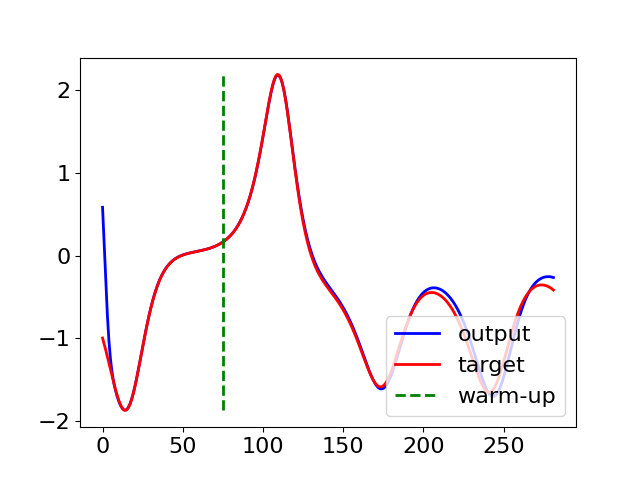
\includegraphics[width=\textwidth]{../Results/Lorenz-63/Figures/RNN-lstm-RDIM_3-N_used_50000-NUM-LAY_1-SIZE-LAY_100-ACT_tanh-ISH_statefull-SL_8-PL_4-LR_0.0001-DKP_1.0-ZKP_1.0-HSPL_300-IPL_200-NL_1-WID_0/prediction_augmend_TEST_33278.png}
			\caption{Prediction of first dimension}
		\end{subfigure}
%		\begin{subfigure}[b]{0.45\textwidth}
%			\includegraphics[width=\textwidth]{../\SixtyThreePath/prediction_TEST_\SixtyThreePathIndexOne_error.png}
%			\caption{Error of first dimension}
%		\end{subfigure}
		\begin{subfigure}[b]{0.45\textwidth}
			\includegraphics[width=\textwidth]{../\SixtyThreePath/prediction_TEST_\SixtyThreePathIndexOne.png}
			\caption{Predictions of all dimensions}
		\end{subfigure}
%		\begin{subfigure}[b]{0.5\textwidth}
		\begin{subfigure}[b]{\textwidth}
			\includegraphics[width=\textwidth]{../\SixtyThreePath/prediction_TEST_\SixtyThreePathIndexOne_contour.png}
			\caption{Contour plot}
		\end{subfigure}
		\caption{Test results for random initial condition \SixtyThreePathIndexOne}
		\label{63:predictions1}
	\end{figure}
	
	\begin{figure}[h]
		\centering
		\begin{subfigure}[b]{0.45\textwidth}
			\includegraphics[width=\textwidth]{../\SixtyThreePath/prediction_augmend_TEST_\SixtyThreePathIndexTwo.png}
			\caption{Prediction of first dimension}
		\end{subfigure}
%		\begin{subfigure}[b]{0.45\textwidth}
%			\includegraphics[width=\textwidth]{../\SixtyThreePath/prediction_TEST_\SixtyThreePathIndexTwo_error.png}
%			\caption{Error of first dimension}
%		\end{subfigure}
		\begin{subfigure}[b]{0.45\textwidth}
			\includegraphics[width=\textwidth]{../\SixtyThreePath/prediction_TEST_\SixtyThreePathIndexTwo.png}
			\caption{Predictions of all dimensions}
		\end{subfigure}
%		\begin{subfigure}[b]{0.45\textwidth}
		\begin{subfigure}[b]{\textwidth}
			\includegraphics[width=\textwidth]{../\SixtyThreePath/prediction_TEST_\SixtyThreePathIndexTwo_contour.png}
			\caption{Contour plot}
		\end{subfigure}
		\caption{Test results for random initial condition \SixtyThreePathIndexTwo}
		\label{63:predictions2}
	\end{figure}

	\FloatBarrier
	\subsection{Lorenz-96}
	\newcommand{\NinetySixPath}{Results/Lorenz-96/Figures/RNN-lstm-RDIM_10-N_used_100000-NUM-LAY_1-SIZE-LAY_100-ACT_tanh-ISH_statefull-SL_8-PL_2-LR_0.0001-DKP_1.0-ZKP_1.0-HSPL_300-IPL_200-NL_1-WID_0}
	\newcommand{\NinetySixPathIndexOne}{25172}
	\newcommand{\NinetySixPathIndexTwo}{50168}
	
		\begin{figure}[h]
		\centering
		\begin{subfigure}[b]{0.45\textwidth}
			\includegraphics[width=\textwidth]{../\NinetySixPath/Loss_total_log.png}
			\caption{Training and validation loss}
			\label{96:loss}
		\end{subfigure}
		\begin{subfigure}[b]{0.45\textwidth}
			\includegraphics[width=\textwidth]{../\NinetySixPath/spectrum_comparison_TEST.png}
			\caption{Power spectrum for test predictions}
			\label{96:spectrum}
		\end{subfigure}
	\end{figure}
	
	\begin{figure}[h]
		\centering
		\begin{subfigure}[b]{0.45\textwidth}
			\includegraphics[width=\textwidth]{../\NinetySixPath/prediction_augmend_TEST_\NinetySixPathIndexOne.png}
			\caption{Prediction of first dimension}
		\end{subfigure}
		\begin{subfigure}[b]{0.45\textwidth}
			\includegraphics[width=\textwidth]{../\NinetySixPath/prediction_TEST_\NinetySixPathIndexOne_error.png}
			\caption{Error of first dimension}
		\end{subfigure}
		%		\begin{subfigure}[b]{0.5\textwidth}
		\begin{subfigure}[b]{\textwidth}
			\includegraphics[width=\textwidth]{../\NinetySixPath/prediction_TEST_\NinetySixPathIndexOne_contour.png}
			\caption{Contour plot}
		\end{subfigure}
		\caption{Test results for random initial condition \NinetySixPathIndexOne}
		\label{96:predictions1}
	\end{figure}
	\begin{figure}[h]
		\centering
		\begin{subfigure}[b]{0.45\textwidth}
			\includegraphics[width=\textwidth]{../\NinetySixPath/prediction_augmend_TEST_\NinetySixPathIndexTwo.png}
			\caption{Prediction of first dimension}
		\end{subfigure}
		\begin{subfigure}[b]{0.45\textwidth}
			\includegraphics[width=\textwidth]{../\NinetySixPath/prediction_TEST_\NinetySixPathIndexTwo_error.png}
			\caption{Error of first dimension}
		\end{subfigure}
		\begin{subfigure}[b]{\textwidth}
			\includegraphics[width=\textwidth]{../\NinetySixPath/prediction_TEST_\NinetySixPathIndexTwo_contour.png}
			\caption{Contour plot}
		\end{subfigure}
		\caption{Test results for random initial condition \NinetySixPathIndexTwo}
		\label{96:predictions2}
	\end{figure}
	